% Copyright 2009, Engine Yard, Inc.
\documentclass{article}

\usepackage{amsfonts} % Math Fonts
\usepackage[linktocpage]{hyperref} % Hyperlinks
\usepackage{graphicx} % Figures
\usepackage{index}    % Indexes
\usepackage[refpage,intoc]{nomencl} % Glossary
\usepackage{multirow} % Row-Spanning in Tabular Context
\usepackage{verbatim} % Comment Environment

% Set Up Main Index and Glossary
\newindex{tech}{tdx}{tnd}{Technology Index}
\newindex{subject}{idx}{ind}{Subject Index}
\makenomenclature

% Handy Definitions
\newcommand{\myfigwidth}{\textwidth}
\newcommand{\myfigheight}{2in}
\newcommand{\resource}{{\sf resource}}
\newcommand{\resources}{{\sf resources}}
\newcommand{\Resource}{{\sf Resource}}
\newcommand{\Resources}{{\sf Resources}}

% Now for the document
\begin{document}

% No Headers Until Actual Content
\pagestyle{empty}

% Copyright 2008, Engine Yard, Inc.
\title{Vertebra: Interim Documentation}
\author{Jayson Vantuyl}

\begin{titlepage}
\begin{center}

{\LARGE Vertebra}\\[0.5cm]
\textsc{Interim Documentation}\\[2.5cm]

Jayson Vantuyl\\[0.5cm]

\textsc{Engine Yard, Inc.}

\vfill


\includegraphics[width=1in]{figs/png/eylogo}\\[\baselineskip]
\copyright 2009, Engine Yard, Inc.\\[\baselineskip]
Released under Creative Commons Public License (Attribution-Noncommercial-No Derivative Works 3.0 United States)\\[\baselineskip]
Details available on the World Wide Web at:\\
\url{http://creativecommons.org/licenses/by-nc-nd/3.0/us/}
\end{center}
\end{titlepage}
 % Title Page

% Set Page Style For Headings
\cleardoublepage
\pagestyle{headings}

\newcommand{\actor}{{\sf actor}}
\newcommand{\actors}{{\sf actors}}
\newcommand{\Actor}{{\sf Actor}}
\newcommand{\Actors}{{\sf Actors}}

\section{Actors}

\subsection{Who Are These Actors?}

\index[subject]{actors|(}
Since Vertebra is about glueing systems together, it is fairly critical to be able to codify and describe exactly what things your are putting together.  With that in mind, an \actor{}\nomenclature{actor}{Vertebra's fundamental unit of code} is the fundamental unit of \textbf{code} in Vertebra.  More colloquially, they are ``where the rubber hits the road''.

Each \actor{} offers various operations that can be done on certain resources.  How exactly this is done is formalized in later chapters.

\subsection{All The World Is A Stage...}

Let's take an example of a bank.  This is a fairly complex organization with many systems in need of management.  Ignoring the higher-level administration of those systems, there are many pieces of code that will directly interface with a number of other systems at a much lower level.  Table \ref{tbl:bank-actors} gives a number of example actors.

\begin{table}
	\begin{center}
		\begin{tabular}{|p{0.35\textwidth}|p{0.55\textwidth}|}
			\hline Actor & Description \\
			\hline
			\hline WidgetTek Drawer Actor & Operates the bank's WidgetTek-brand cash drawers \\
			\hline SprocketInc Drawer Actor & Operates the bank's SprocketInc-brand cash drawers \\
			\hline Vault Actor & Operates the bank's vault control mechanism \\
			\hline Check Reader Actor & Operates the bank's check readers \\
			\hline ACH Dial-In Actor & Operates dial-in lines used by the bank's merchant services credit card machines \\
			\hline ATM Actor & Controls secure leased lines to various ATMs \\
			\hline Ledger Access Actors & Provides access to systems that handle and distribute ledger data throughout the bank \\
			\hline Optical Storage Actor & Provides access to optical storage used for archiving check scans and bank records \\
			\hline Alarm System Actor & Interfaces with security alarm \\
			\hline Collect-o-matic Actor & Interfaces with an IVR system that harasses delinquent loan customers \\
			\hline
		\end{tabular}
	\end{center}
	\caption{Example Actors In A Bank}
	\label{tbl:bank-actors}
\end{table}

This list of \actors{} is obviously fanciful and incomplete, but it should indicate that the focus of \actors{} is the programmer.

It is worth noting that, just like real-world code, sometimes two \actors{} perform the same function for different pieces of equipment.  This is intentional and should make \actors{} the natural point to create consistent interfaces.  It is our belief that this aids in refactoring as well, since it keeps the focus on making access similar resources uniform.

Whatever way makes sense for a programmer to encapsulate the code that really does the work, can be factored into \actors{}.  This is where all of the concerns about where code runs or how it works is addressed.  This is where it is necessary to deal directly with the vagaries of hardware access, user interfaces, and all of the details that crop up in a large system.  The rest of Vertebra handles knitting them together at a much higher level.
\index[subject]{actors|)}
% Copyright 2008, Engine Yard, Inc.
\newcommand{\agent}{{\sf agent}}
\newcommand{\agents}{{\sf agents}}
\newcommand{\Agent}{{\sf Agent}}
\newcommand{\Agents}{{\sf Agents}}

\section{Agents}

\subsection{Agent Who?}

\index[subject]{agents|(}
While \actors{} are the fundamental unit of         extbf{code}, \agents\nomenclature{agent}{Vertebra's fundamental unit of deployment} are the fundamental unit of         extbf{deployment}.  A dizzying array of different issues must be managed when deploying code.  Most programmers are ill-equipped to address these issues.  They are primarily the domain of administrators.  By removing to need for these two groups to depend wholly on one another, we can reduce some of the mismatch that invariably must be overcome to implement a deployable system.

The primary deployment issues we address are:

\begin{itemize}
        \item security
        \item provisioning
        \item configuration
\end{itemize}

Mixing the above needs with the actual code would only serve to interfere with the purpose of that code while giving a haphazard treatment to those same needs.  Vertebra neatly handles the above by grouping \actors{} into \agents{}, which have varying groups of \actor{} code, custom configuration, and an array of provisioning needs.

\subsection{Your Papers Seem To Be In Order...}

\Agents{} are where credentials first appear in Vertebra.  Controlling who runs a certain piece of code and what power they have over the system as a whole is critical.  The \agent{} is the beginning and end of identification.  With this single building block, we can express a wide variety of permissions and security roles.

\subsection{Who Am I?}

\Agents also provide the basic provisioning information that gives \actors{} context.  Without knowing where it is running, an \actor{} can't flexibly determine how it is supposed to operate.  The \agent{} level is where \actors{} are provided with this context.

\subsection{What Do I Do?}

Just because the \actors{} know how to handle a certain piece of equipment doesn't mean that they can magically infer everything necessary.  The \agent{} also can provide a base-level of configuration that doesn't make sense to anyone else.

\subsection{Why Here?}

I can hear the sound of thousands of administrators quaking in fear.  Many of them have a love (or even obsession) with provisioning, securing, and configuring centrally over the network.  The thought is that this eases administration by centralizing those concerns.

In the Cloud, we have discovered that this centralization is directly at odds with reliability and scalability.  Anyone who has witnessed the carnage when database servers or authentication servers go offline will appreciate that some things should be configured locally.  This level of configuration allows you to do so--which should, in turn, allow your system to make a best-effort in the event of catastrophe.  Similarly, you'll never have to worry about scaling or replicating your LDAP server or RADIUS server.

That said, Vertebra does provide a central configuration store in Entrep\^ot.  While we would love for all of your critical configuration to go there, we recognize that some information just makes sense at the leaves of your network, not somewhere in the center.  Our core data storage specification is detailed later\footnote{see page \pageref{ref:core-data-storage}}.

\index[subject]{agents|)}

\newcommand{\resource}{{\sf resource}}
\newcommand{\resources}{{\sf resources}}
\newcommand{\Resource}{{\sf Resource}}
\newcommand{\Resources}{{\sf Resources}}

\section{Resources}

\index[subject]{resources|(}

\subsection{What Is A Resource?}

\index[subject]{resources!definition}

Perhaps the most fundamental concept in Vertebra is that of a \resource\nomenclature{resource}{Vertebra's fundamental unit of addressing}.  Conceptually, \resources{} are the fundamental unit of \textbf{addressing} in Vertebra.  In the abstract, a \resource{} represents something that matters to your application.  It might be a certain piece of data, a certain point of control, or a certain type of behavior.  Vertebra doesn't give it any meaning, your application does.

\index[subject]{resources!hierarchy}Just like concepts in your application, \resources{} can have relationships to each other.  In order to keep things relatively manageable, Vertebra's understanding of relationships is limited to a strict hierarchy.  In object-oriented parlance, it is the {\bf is-a} relationship embodied by a single inheritance model.  More formally, this means that any \agent{} that can be identified by a certain \resource, should also be identified by any ancestors of that \resource{}.

Given this framework, a rich variety of concepts should be representable.  A simple example of a set of resources are given in table \ref{tbl:res-philosopher}.  A visualization of the hierarchy they produce is given in figure \ref{fig:res-example2}.  Note the many dissimilar concepts are represented in this \resource{} hierarchy:

\begin{itemize}
	\item Citizenship
	\item Geography
	\item Professional Trades
	\item Language Fluency
\end{itemize}

In the example, we have used a path notation which lists all of the ancestor \resources{}, prepended to the \resource{} directly offered.  So the the entry ``{\sf/speaker/greek}'' indicates that Socrates speaks greek, which also implies that he speaks at all.

\begin{table}
	\begin{center}
		\begin{tabular}{| c | l |}
			\hline
			  Philosopher & Resources \\
			\hline
			\hline
			  \multirow{5}{*}{Socrates}              & /citizen/greece/athens \\
			                                         & /philosophy/classical\_greek \\
			                                         & /service/philosopher \\
			                                         & /service/stonemasonry \\
			                                         & /speaker/greek \\
			\hline
			  \multirow{5}{*}{Aristotle}             & /citizen/greece/athens \\
			                                         & /philosophy/aristotelianism \\
			                                         & /philosophy/peripatetic \\
			                                         & /service/philosopher \\
			                                         & /speaker/greek \\
			\hline
			  \multirow{9}{*}{Cicero}                & /citizen/rome \\
			                                         & /philosophy/stoic \\
			                                         & /service/lawyer \\
			                                         & /service/orator \\
			                                         & /service/philosopher \\
			                                         & /service/political\_theorist \\
			                                         & /service/statesman \\
			                                         & /speaker/greek \\
			                                         & /speaker/latin \\
			\hline
			  \multirow{8}{*}{Thomas Aquinas}        & /citizen/sicily \\
			                                         & /philosophy/scholasticism \\
			                                         & /service/political\_advisor \\
			                                         & /service/philosopher \\
			                                         & /service/lecturer \\
			                                         & /service/theologian \\
			                                         & /service/latin \\
			                                         & /speaker/italian \\
			\hline
			  \multirow{4}{*}{Nietzsche}             & /citizen/prussia \\
			                                         & /philosophy/weimar\_classicism \\
			                                         & /service/philosopher \\
			                                         & /speaker/german \\
			\hline
		\end{tabular}
	\end{center}
	\caption{Resources Possibly Offered By Various Famous Philosophers}
	\label{tbl:res-philosopher}
\end{table}

\begin{figure}
	\begin{center}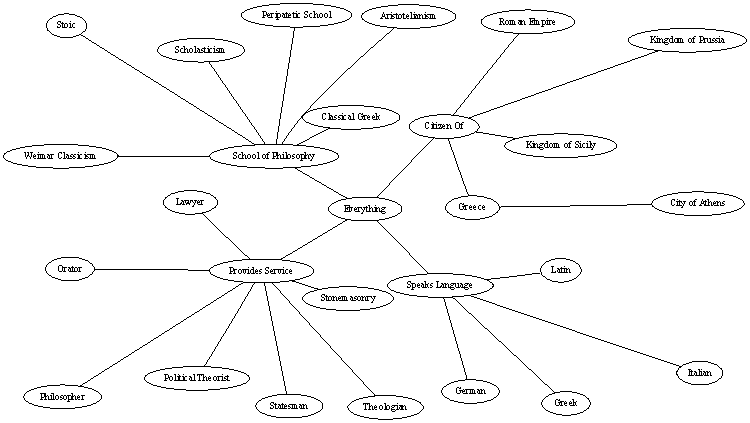
\includegraphics[width=\myfigwidth,height=\myfigheight,keepaspectratio]{figs/dot/res_example2}\end{center}
	\caption{Visualization of the Resource Hierarchy}\label{fig:res-example2}
\end{figure}

\subsection{Resources Are Groups Of Agents}

Hopefully it is evident from the above discussion that \resources{} are never actually realized \emph{per se}.  There is never a specific data structure or thing that can be said to be a \resource.  Instead, a \resource{} is more like a description or a tag.  What is significant about it is the set of things that it identifies.

Consequently, it's very useful to think of resources as sets of \agents{}.  \Agents{} that have something you want!  That's convenient, because it is very easy to use common techniques to visualize groups of \agents{} and their relationships.  An example using a Venn Diagram is shown in figure \ref{fig:res-example1}.

\begin{figure}
	\begin{center}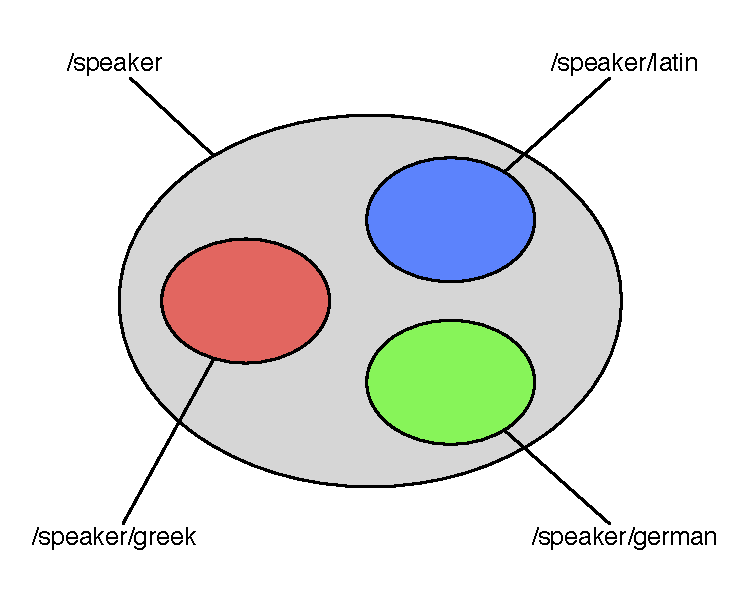
\includegraphics[width=\myfigwidth,height=\myfigheight,keepaspectratio]{figs/omnigraffle/res_example1}\end{center}
	\caption{Venn Diagram of a Resource Hierarchy}\label{fig:res-example1}
\end{figure}

\subsection{Resource Advertisement}

\index[subject]{advertising|see{resources}}
\index[subject]{resources!advertising|(}

In the more concrete sense, an \actor{} is said to ``provide'' a \resource{}.  When an \actor{} ``provides'' a \resource{} it causes any \agent{} that is configured with that \actor{} to ``advertise'' the same \resource{} (or perhaps an ancestor of it).  This causes requests to operate on that \resource{} to be directed to that \agent{}, which subsequently directs it to the appropriate \actor{}.

TODO: Put a bank example here.

\subsection{The Root Resource}

There is one final bit of errata.  It may not be so obvious from the above example, but all resources descend from a common, catch-all ancestor---the {\sf root} resource.  In our path notation, it is identified by the path ``{\sf /}''.

The root resource is rarely advertised on its own, but can be very useful when \resources{} are used for security and discovery purposes.

\subsection{The Advertising Process}

You may have noticed that I brushed over the details of ``advertising''.  Unfortunately we don't have all of the basics necessary to discuss advertising.  What I can tell you is that the \agent{} sends a message to the Vertebra security agent listing which \resources{} are offered.  We'll cover some more of the specifics in \ref{ref:direct-ops}.

\index[subject]{resources!advertising|)}

\index[subject]{resources|)}

\section{Discovery}

\index[subject]{discovery|see{resources}}
\index[subject]{resources!discovery of|(}

\subsection{The Unique Issues of the Cloud}

Now that we have built a flexible system for representing the \resources{} that matter to our applications, it is important to be able to work with them.  This is where the Cloud diverges from most programming endeavors.  On the smaller scale, most programmers spend much of their time fighting with how their data is represented.

Holy wars are waged over such cherished technologies as relational databases, document schemas, object-relational mappers, and interchange formats.  \Resources{} allow Vertebra to be fairly agnostic to these issues.  We don't care what you are exchanging, we just want to help it get there.

\subsection{The Cloud Makes ``Where?'' Hard}

That brings up the unique problem of scaling.  In a large enough deployment, it is very expensive to have anything centralized.  Most people focus on making increasingly efficient centralized components--hoping to push off the scalability problems as far as possible.  In Vertebra, we accept that you may or may not be centralized, but that your primary concern is locating that data--or service, or employee.  \Resources{} save the day in that respect.

For this to be useful, Vertebra provides a facility called ``discovery''.  Discovery allows you to ask for some group of agents by giving their fingerprint as a set of resources.  Vertebra will then handle distributing your request to all of the appropriate places for it to go.

\subsection{Scatter-Gather Computing}

To make this work, \agents{} advertise their membership in the groups for which their \actors{} provide \resources{}.  This makes it possible for any requesters to discover the other \agents{} in the cloud that can fulfill their requests.  With discovery, it's easy to spread out data by discovering the destination (i.e. \emph{push} or \emph{scatter}).  Conversely, it's also easy to collect data by discovering the source (i.e. \emph{pull} or \emph{gather}).  In this way it is possible to offer facilities similar to ``publish-subscribe'' systems, but potentially with services instead of data---potentially even for legacy services that are otherwise difficult to integrate with such systems.

\subsection{Discovering A Teller}

TODO: Provide an extension of the bank example that illustrates discovery.  Possibly do so by putting a bank example in the resources section, to give a more comprehensive example set.

\subsection{The Discovery Process}

Just like ``advertising'', the specifics of ``discovery'' will be deferred until \ref{ref:direct-ops}.  In the same vague language used before, the \agent{} sends a message to the Vertebra security agent requesting another \agent{} which offers the appropriate \resources{}.

\index[subject]{resources!discovery of|)}

\newcommand{\operation}{{\sf operation}}
\newcommand{\operations}{{\sf operations}}
\newcommand{\Operation}{{\sf Operation}}
\newcommand{\Operations}{{\sf Operations}}

\newcommand{\scope}{{\sf scope}}
\newcommand{\scopes}{{\sf scopes}}
\newcommand{\Scope}{{\sf Scope}}
\newcommand{\Scopes}{{\sf Scopes}}

\newcommand{\single}{{\sf single}}
\newcommand{\Single}{{\sf Single}}

\newcommand{\all}{{\sf all}}
\newcommand{\All}{{\sf All}}

\section{Overview}

Now that we have a number of useful abstractions, it's time to do something with them.  For this purpose, Vertebra has \operations{}.  The \operation{} is the fundamental unit of \textbf{work} in Vertebra.  At any instant, they tie the pieces together to make something happen.

Specifically, when an \operation{} is issued, the system discovers \agents{} that offer the appropriate \resources{}, then operation is dispatched to those \agents{}.  The \agents{} further dispatch the \operations{} to the appropriate \actors{} which actually do the work.  Finally, the responses stream back to the \agent{} that made the request for the \operation{}.
% Copyright 2008, Engine Yard, Inc.
\section{Scope}

\subsection{Selecting Agents}

\index[subject]{scope|see{operations}}
\index[subject]{operations!scope|(}

Exactly which agents are selected for an \operation{} is determined by the \resources{} in the \operation{} and the \scope{}.  Thus, \scope{} determines the behavior of \textbf{agent selection} in Vertebra.  While it may not be initially obvious, different modes of selection provide the building blocks for implementing a number of useful scenarios which are detailed later.

\subsection{Single Scope}

\index[subject]{operations!scope!single}
The simplest \scope{} that Vertebra provides is the \single{} \scope{}. The purpose of the \single{} \scope{} is to ensure that the \operation{} is executed by exactly one \actor{}, exactly once, somewhere in the Cloud.

To dispatch a \single{} scoped \operation{}, the client code discovers \agents{} capable of providing it, then randomly iterate through them.  Each iteration, the \operation{} is dispatched to the selected \agent{}.  If it executes, iteration stops.  If it can't perform the operation, iteration continues to the next \agent{}.  If all \agents{} refuse the \operation{}, the \operation{} blocks and retries at a later point.

\subsection{All Scope}

\index[subject]{operations!scope!all}
The next \scope{} that Vertebra provides is the \all{} \scope{}.  The purpose of the \all{} \scope{} is to ensure that the \operation{} is executed by as many \actors{} as can be reached in the Cloud.

To dispatch an \all{} scoped \operation, the client code discovers \agents{} capable of providing it, then dispatches to all of them simultaneously.  Any or all of the \operations{} could fail.  It may even be that no \agents{} provide the \operation{}.

\index[subject]{operations!scope|)}

% Copyright 2008, Engine Yard, Inc.
\section{Direct Operations}

\label{ref:direct-ops}
\index[subject]{operations!direct|(}
\index[subject]{direct operation|see{operations}}

\subsection{The Chicken and the Egg}

Given all of the talk of discovery and dispatch, there is an exception to those rules.  There are some cases where discovery is not necessary or possible.  The primary case we're concerned with is the \operations{} of advertisement and discovery themselves.

Rather than building a special protocol for doing these \operations, we just use the normal \operation{} behavior, without the discovery step.  We call these ``direct'' \operations{}.

\subsection{Scope In Direct Operations}

\index[subject]{operations!direct!scope in}

Scope in a direct \operation{} is almost unused.  The only aspect of scope that is important is the completion semantics.  That is, for \single{} scope, the operation must be dispatched to exactly one actor, but the \all{} scope, zero or more actors may handle a request.

\index[subject]{operations!direct|)}

% Copyright 2008, Engine Yard, Inc.
\section{General Operations}

\index[subject]{operations!general}
\index[subject]{general operation|see{operations}}

\subsection{Structure}

Everything that happens in Vertebra is an \operation{}.\nomenclature{operation}{Vertebra's fundamental unit of work}  Conceptually, \operations{} are the fundamental unit of         extbf{work} in Vertebra.  With the exception of some infrastructure (i.e. direct \operations{}), they are all general \operations{}.  A general operation takes place in a few phases that provide various execution guarantees.

An operation consists of the components listed in table \ref{tbl:op-parts}.

\begin{table}
        \begin{center}
                \begin{tabular}{|p{0.35        extwidth}|p{0.55        extwidth}|}
                        \hline         extbf{Component} &         extbf{Description} \\
                        \hline
                        \hline Scope      & a string that determines the dispatch and completion requirements of the operation \\
                        \hline Type       & a string that determines which operation is dispatched \\
                        \hline Parameters & a mapping of parameter keys (strings) to various parameter datatypes \\
                        \hline
                \end{tabular}
        \end{center}
        \caption{Operation Components}
        \label{tbl:op-parts}
\end{table}

\subsection{Operation States}

The life of an operation goes through various states, as shown in figure \ref{fig:op-states}.

\begin{itemize}
        \item         extbf{New} --- Operation has been requested but has not started.
        \item         extbf{Ack} --- Operation has been acknowledged as allowed and may be starting.
        \item         extbf{Nack} --- Operation has been denied due to security policy, operation-specific issue, due to load, or due to old discovery information.
        \item         extbf{Run} --- Operation is executing.
        \item         extbf{Done} --- Operation has finished.
        \item         extbf{Error} --- Operation has failed at an application level.
\end{itemize}

\begin{figure}
        \begin{center}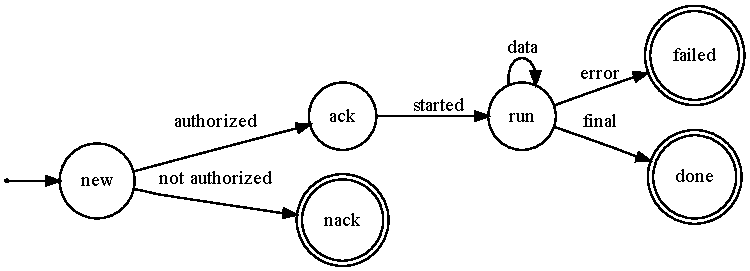
\includegraphics[width=\myfigwidth,height=\myfigheight,keepaspectratio]{figs/dot/op_states}\end{center}
        \caption{Operation States}
        \label{fig:op-states}
\end{figure}

% Copyright 2008, Engine Yard, Inc.
\section{Core Data Storage}

\subsection{Requirements}

\label{ref:core-data-storage}To orchestrate services in the cloud, information of a certain character must be stored and queried.  A data store for Vertebra needs to have a few characteristics:

\begin{itemize}
        \item it should be fault-tolerant
        \item it should be horizontally scalable
        \item it should be keyed similarly to operation discovery
        \item it should have values that easily adapt to become input to operations
        \item it should have a versioning capability
\end{itemize}

The Vertebra implementation provides a data store with these properties\footnote{TODO: versioning isn't done yet.} in the form of Entrep\^ot.

\subsection{Data Format}

Entrep\^ot is, at the highest level, a hash-table.  It simply maps keys to values.  The structure of these keys and values are such that they fit well into the rest of the Vertebra system.

\subsubsection{Keys}

Keys are made up of sets of \resources{}.  This allows for records to be discovered in a similar way that \agents{} are discovered.

\subsubsection{Values}

Values are exactly the same structure as the parameters to an operation.  Functionally they are equivalent to a mapping of parameter keys to values.

\subsubsection{Records}

Each mapping is called a record.  Records are represented as a hash containing:

\begin{description} 
        \item[keys] which maps to a mapping of key names to \resources{}
        \item[values] which maps to a mapping that holds whatever data is being stored
\end{description}

\subsection{Operations}

\subsubsection{Store}

To store a value in an Entrep\^ot data store, do an operation of type ``store'' with scope \single{}.  This guarantees that exactly one copy of the entry is stored.  The parameter mapping for this operation should be the record.

To delete a value in Entrep\^ot, store an empty value.  If a record is replaced (or deleted), the previous record is returned as data.

\subsubsection{Fetch}

To retrieve a value, there are two options depending on the type of query you're attempting.

To find all records which have a key that contains the query keys, use an \operation{} of type ``fetch\_superset''.  To find all records which have a key that is contained by the query keys, use an \operation{} of type ``fetch\_subset''.  In either case, the queries should be made with a parameter named ``keys''.

The data returned will consist of a mapping containing records of the form used in the Store \operation{}.

\subsection{Caveats}

Entrep\^ot makes its best effort to update and delete values.  However, it is not currently completely resilient.  This will be addressed later when versioning is supported.  The current shortcomings are mostly of concern in federated settings where there is a significant likelihood that communication between two servers is significant.

Provisioning is also a concern, since an Entrep\^ot \agent{} will not be discovered unless it contains resources for all of the keys in a request.  This should be handled by direct \operations{} for the initial store.


\end{document}
